
% AUTHOR_body.tex
% Prepared by C. Pinon (cjpinon@implicature.xyz) for EISS 13 (see
% https://implicature.xyz/eiss13/)
% 2020-02-02

% Please use this file (which you should rename) for the main ("body")
% part of your paper. Be sure to compile the master file, not this one.

% Put your main text here. Recall that the references are in a separate
% file. And recall also that "\begin{document}" and "\end{document}"
% have already been inserted, which means that you can begin immediately
% with the first section.

\section{Introduction}\label{sec:1}

These are general instructions for writing a paper for EISS 15, covering basic requirements of the text as far as typesetting is concerned.

%In this paper, we will show how semantics and pragmatics reduce to
syntax (or the other way around, see \citealt{Kamp:1973,Searle:1964}) \ldots 

\section{Basic linguistic typesetting}

Here, we show how frequently needed linguistic elements can be typeset in \LaTeX. These instructions should cover most of your needs. 

\subsection{Linguistic examples with glosses and translations}

For examples, use \textbf{linguex}, and for glossing morphological categories, please refer to the Leipzig Glossing Rules.

\ex. Swiss German \citep[][346]{hodler69}
\gll win er der Namen Gottes het usgsprochn-a ghabe\\
when he the name.\textsc{m.sg} God.\textsc{gen} has pronounced-\textsc{m.sg} had\\
`once he had pronounced the name of God'

\Next shows how you can typeset examples with several subexamples. Please avoid, if at all possible, examples that are cut from their translation. You may want to force a new page, if this cannot be avoided. In order to refer back or forth to an example, you can either do it like \ref{ex:1} and \ref{ex:2}, or rather with the shorthands \Next[c] or \Last. Either will work, but only the first version will require that you add a \emph{label} to the example, as we have done below.


\ex. \label{ex:1}\a. \label{ex:2}First example
\b. Second
\bg. Dies ist ein schönes Beispiel mit einer Glose.\\
This is a beautiful example with a gloss.\\
\a. `Some translation'
\b. `Some other'
\z.
\b. Fourth

You can refer back to examples like \ref{ex:1} and \ref{ex:2}.

\subsection{IPA \& Unicode}
\label{sec:IPA}

The final version of this paper will be compiled using LuaLateX. This engine (similar to \texttt{xelatex}) gives you direct access
to the entire rich set of Latin script unicode characters. This includes (but is by no means limited to) IPA.
You may even use TIPA macros to input IPA characters, as an
alternative to inputting unicode characters directly, e.g.
\verb|\textturna\textipa{ES}| will yield \textturna\textipa{ES},
correctly using your main font. 

\subsection{Trees}

In order to make trees, use the \textbf{forest} package.

% LaTeX doesn't care how you arrange the tree in the source code, but for your own sake, you want probably want to write something as follows:
\ex. \begin{forest}
[S 
  [DP [D [ Ce\\\footnotesize{This} ] ]
      [NP [AP [A [ petit\\\footnotesize{small} ] ] ]
          [N [ arbre\\\footnotesize{tree} ] ] ] ]
  [VP [V [ est\\\footnotesize{is} ] ]
      [AP [AdvP [Adv [ très\\\footnotesize{very} ] ] ]
          [A [ joli\\\footnotesize{nice} ] ] ] ] ]
\end{forest}

You can also make a more involved example, with arrows, as is illustrated in \NNext. Ideally, you would want to avoid big spaces (you can adjust the size of the tree, if this is necessary, as we have done in \Next for \Last). 

\ex. \small{
\begin{forest}
[S 
  [DP [D [ Ce\\\footnotesize{This} ] ]
      [NP [AP [A [ petit\\\footnotesize{small} ] ] ]
          [N [ arbre\\\footnotesize{tree} ] ] ] ]
  [VP [V [ est\\\footnotesize{is} ] ]
      [AP [AdvP [Adv [ très\\\footnotesize{very} ] ] ]
          [A [ joli\\\footnotesize{nice} ] ] ] ] ]
\end{forest}
}


\ex.  \label{ex:rp-structure} 
\footnotesize{%
\begin{forest} for tree={l=10mm, l sep=0}
   [AuxP, name=top 
      [beP [RP 
              [DP [John] ] 
              [R$'$ [withP  
                       [RP [DP [hair] ] 
                           [R$'$ [AP [VP ] 
                                     [A [ colored, name=cellar ] ] ] 
                                 [R] ] ] 
                        [with, name=source] ] 
                    [R, name=c1] ] ] 
            [be, name=c2]   ]  
      [Aux [ has ] ] ]
    % and now, we draw some arrows  
   \draw[->,color=red,very thick,dotted] (source) to[out=east,in=south east] (c1);
   \draw[->,color=blue,ultra thick,dashed] (c1) to[out=east,in=south east] (c2);
   \draw [-{Latex[length=2.5mm]},color=purple,ultra thick,%
          postaction={decorate,decoration={text along path,%
          text align=center,raise=-2.5ex, text color = purple,%
          text={{Because why the hell not}}}}] (cellar) to[out=east,in=east] (top);
\end{forest}}


\subsection{AVMs}

For avms, we use \textbf{langsci-avm}.

\ex. \avm{[ attr1 & \1\\
attr2 & \2[attr3 & val3\\
attr4 & val4] ]}

You can combine \textbf{forest} and \textbf{langsci-avm}:

\ex. \begin{forest}
[A [B] [{\avm{[attr1 & val1\\
attr2 & val2\\
attr3 & val3]}} ] ]
\end{forest}l

\subsection{Tables}

For tables, we use the \textbf{booktabs}-environment, as illustrated in Table \ref{tab:article-systems}. 



%\textbf{Question: do we insist that tables are put in a table-environment?}

\begin{table}
 \centering
 \begin{tabular}[t]{lr}
  \toprule
  Type of language                     & Number \\
  \midrule
  No articles at all                   & 198    \\
  Both indefinite and definite article & 154    \\
  Definite, but no indefinite article  & 89     \\
  Indefinite, but no definite article  & 40     \\
  \midrule
  Total                                & 481    \\
  \bottomrule                                       
\end{tabular}
  \caption{Article Systems in the World's Languages according to \emph{WALS}}
  \label{tab:article-systems}
\end{table}

\subsection{Figures}

And finally, you can also add figures. Figures are floats in \LaTeX{}, so they might end up on another page. When adding a figure, please make sure that the picture is in a high enough resolution (we recommend 300dpi or more), and that you have the right to include the picture.

\begin{figure}
    \centering
    % you might need to adjust the width of the picture
    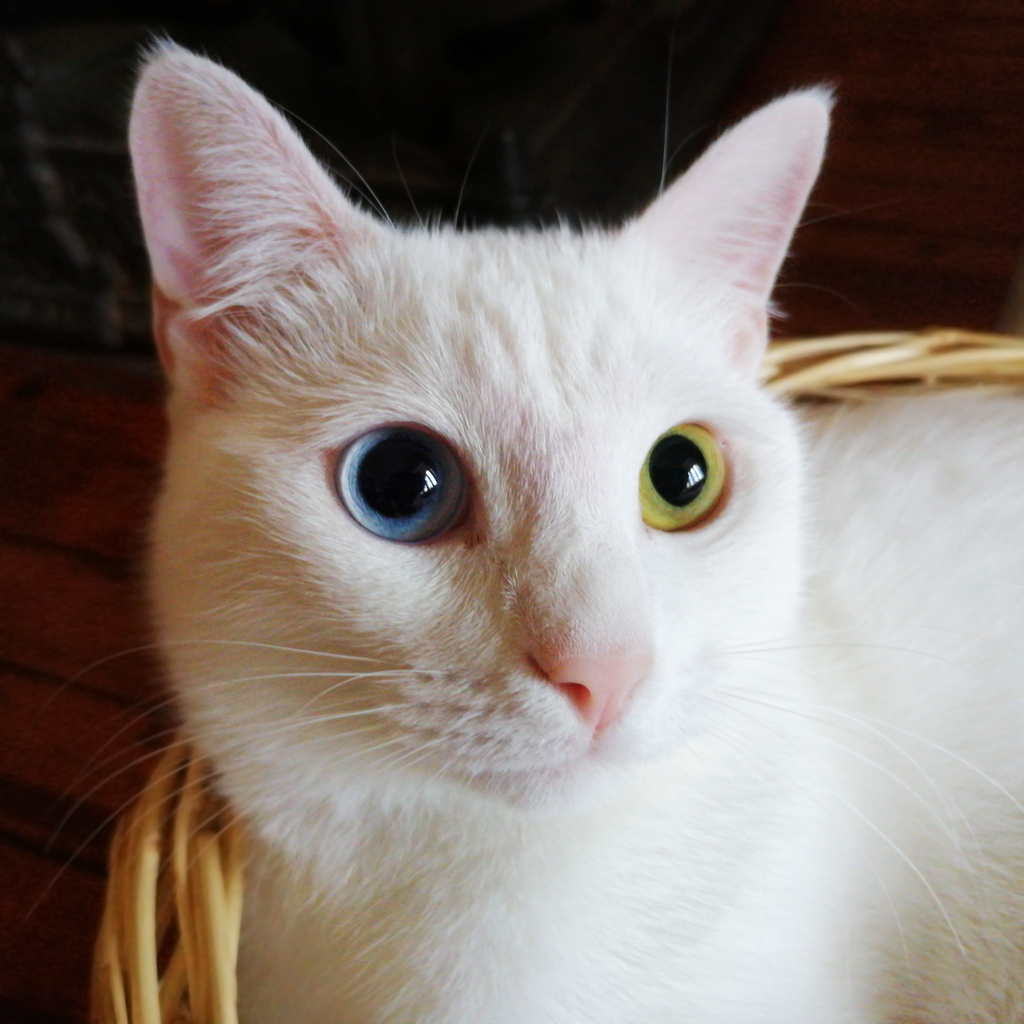
\includegraphics[width=0.4\textwidth]{cat.png}
    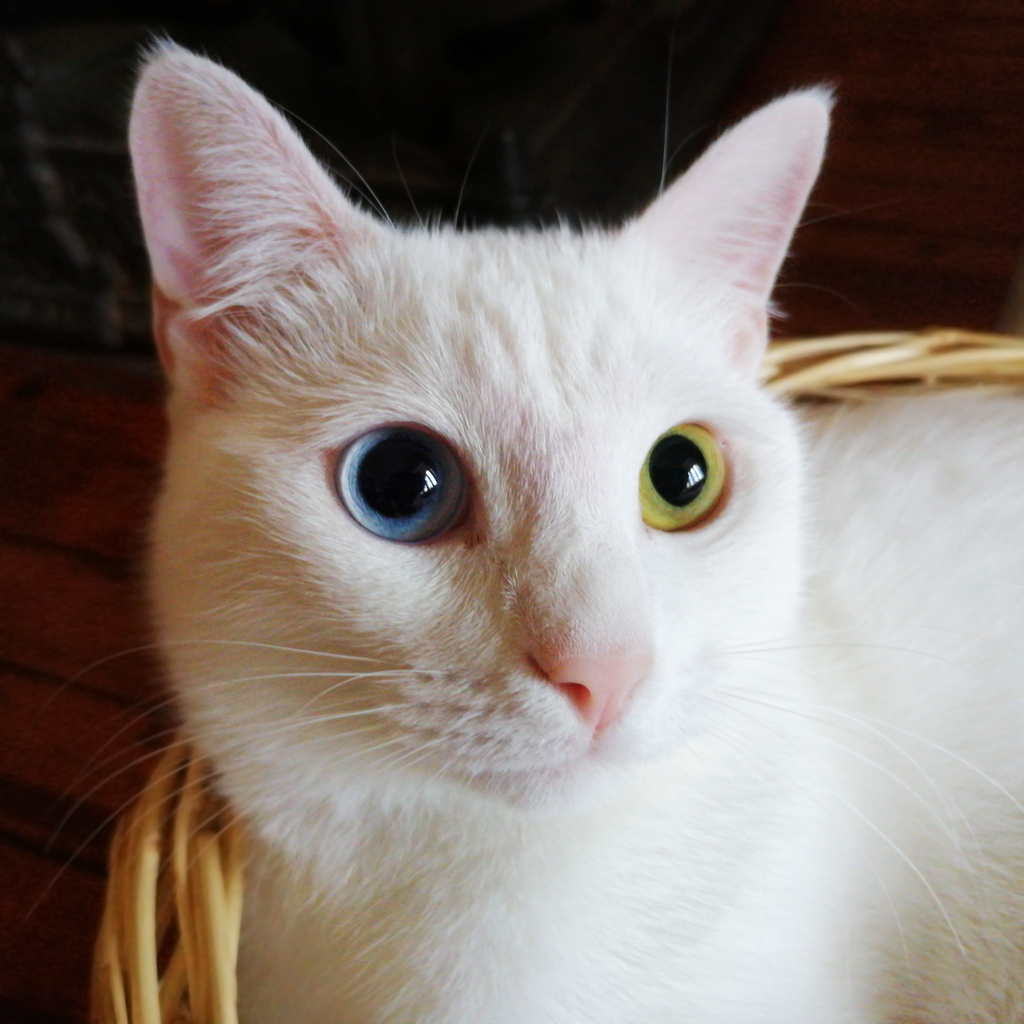
\includegraphics[width=0.4\textwidth]{cat.png}
    \caption{A cute cat and its identical twin (not sure if this is relevant)}
    \label{fig:my_cat}
\end{figure}

As usual, you can refer back to Figure \ref{fig:my_cat}.\footnote{Source of the cat: \href{https://commons.wikimedia.org/wiki/File:VAN_CAT.png}{https://commons.wikimedia.org/wiki/File:VAN\_CAT.png}.}

\section{Dealing with references}

%For references, we use \textbf{biblatex}. You can use the format familiar familiar from natbib. For instance, it is no problem to say that \citet[451]{Szadrowsky:1936} claims something, but I am not sure whether \citet[70]{Kamp:1973} would agree (or \citealt[50]{Searle:1964}, by that matter).
In our style file, we use BibLaTeX, rather than the older BibTex. As a consequence, you can use unicode encoding in your BIB file, and you are not restricted to the ASCII-range.

Therefore, you can write directly:

\begin{verbatim}
title =  {Über die Sprache und Weisheit der Indier},
\end{verbatim}

rather than the older, escaped version:

\begin{verbatim}
title =  {\"{U}ber die Sprache und Weisheit der Indier},
\end{verbatim}

The latter will continue to work.

We use BibLaTeX with the \texttt{natbib} switch, and thus, all \texttt{natbib} commands  should work and behave as expected. You can continue to use the following and more:

\begin{verbatim}
  \cite{chomsky1995}   % discouraged by natbib
  \citet[12]{chomsky1995}
  \citep[see, e.g.][12]{chomsky1995}
  \citealt[12]{chomsky1995}
  \citealp*{chomsky1995}
\end{verbatim}

\subsubsection*{No BibLaTeX warnings}

When running BibLaTeX on your BIB file, there should be \textbf{no warnings or errors whatsoever}. Please pay attention to the BibLaTeX compilation log to verify this.

\subsubsection*{Don't abbreviate names}

Every entry in your BIB file should include \textbf{the names of the authors and editors as they appear on the work in question} -- please don't abbreviate any author's or editor's name yourself.

For example, the author of the book \emph{Semantic interpretation in generative grammar} is given as "Ray S. Jackendoff". If you want to cite this book, then the corresponding entry in your BIB file should contain the following author field:

\begin{verbatim}
author = {Jackendoff, Ray S.},
\end{verbatim}

In this example, you \textbf{shouldn't} abbreviate ''Ray S.'' as ''R. S.'' or ''Ray'' or ''R.''.

\subsubsection*{Don't force unnecessary capitalization in titles}

Since there are different bibliographic styles for how titles of works of different types are capitalized, please don't force unnecessary capitalization in titles of works in your BIB file, for otherwise a bibliographic style (which is determined by a bibliographic style file) won't be able to change this.

For example, if you want to cite the book \emph{The sound pattern of English}, then the corresponding entry in your BIB file should contain the following title field (following the convention known as \href{https://en.wikipedia.org/wiki/Letter_case#Title_case}{Title case}):

\begin{verbatim}
title = {The Sound Pattern of {English}},
\end{verbatim}

If the title is given in this way, then ''English'' will be capitalized, whereas ''Sound'' and ''Pattern'' may but need not be capitalized, which allows the bibliographical style file to decide, depending on the chosen bibliographic style. (Note that ''The'' will necessarily be capitalized because it is the first word of the title.)

Any other variation in how this title is given could lead to undesirable results.

If you enclose in brackets only the first letter of the word you wish to capitalize, this will interfere with correct kerning between the first letter and the rest of the word. So, avoid the following:

\begin{verbatim}
title = {The Sound Pattern of {E}nglish},
\end{verbatim}

Another common mistake would be to write the title as follows:

\begin{verbatim}
title = {{The Sound Pattern of English}},
\end{verbatim}

But this would force the capitalization of ''Sound'' and ''Pattern'', which may contradict the chosen bibliographic style.

Similarly, do not write the title as follows:

\begin{verbatim}
title = {The sound pattern of English},
\end{verbatim}

In this case, the problem is that this wouldn't force of the capitalization of ''English'', which would be incorrect, and it also wouldn't allow for the capitalization of ''sound'' or ''pattern'', which again may contradict the chosen bibliographic style.

Similarly, do not write the title as follows:

\begin{verbatim}
title = {The sound pattern of English},
\end{verbatim}

In this case, the problem is that this wouldn't force of the capitalization of ''English'', which would be incorrect, and it also wouldn't allow for the capitalization of ''sound'' or ''pattern'', which again may contradict

\subsubsection*{References in languages other than English}

Naturally, what was said above applies to titles of works in English. Other languages, for example, French, don't have a tradition of title case, and in the case of German, the orthography requires all nouns to be capitalized.

In such cases, do not force the capitalization of all common nouns by enclosing it in brackets, but rather add a special \texttt{LANGID} identifier, and let BibLaTeX do the rest:

\begin{verbatim}
 title =  {Über die Sprache und Weisheit der Indier},
 langid = {german},
\end{verbatim}

\begin{verbatim}
 title =  {Cours de linguistique générale},
 langid = {french},
\end{verbatim}

\section{Limitations}

As of now, we only support 5 authors. If your paper has more than 5 authors, please get in touch with us.

You can no longer compile to dvi. This is not something we intend to change.


\renewcommand{\Abbrevs}{List here the abbreviations you used in your paper. For a list of standard abbreviations, refer to the \href{https://www.eva.mpg.de/lingua/resources/glossing-rules.php}{Leipzig glossing rules}. Sort alphabetically, and indicate the abbreviations in the following format: \textsc{gen} = genitive, \textsc{m} = masculine, \textsc{sg} = singular.}%

%%%%%%%%%%
%% The official end of this file
%%%%%%%%%%

%%% Local Variables:
%%% mode: lualatex
%%% TeX-master: "main"
%%% End:
